Salgssystemet fungerer først og fremmest via et Kasseapparat med et grafisk touch interface, herfra kan Ekspedient sælge varer til en kunde og tage imod betaling herfra. 

Kasseapparatet sender/henter data til/fra CentralServer der yderligere kommunikere med databasen, dette gør at Kasseapparatet kan modtage et produktkatalog fra, og få gemt et salg, i databasen. 

Superbruger har igennem et grafisk interface adgang til Administrationssystem. Herfra kan Superbruger tilføje, slette og redigere produkter og produktkategorier i produktkataloget. Dette betyder at Administrationssystemet også har en forbindelse til CentralServer.

CentralServer sørger for al kommunikation med databasen og at håndtere al kommunikation til og fra alle instanser af Administrationssystem og Kasseapparat.


\begin{figure}[!h]
    \centering
    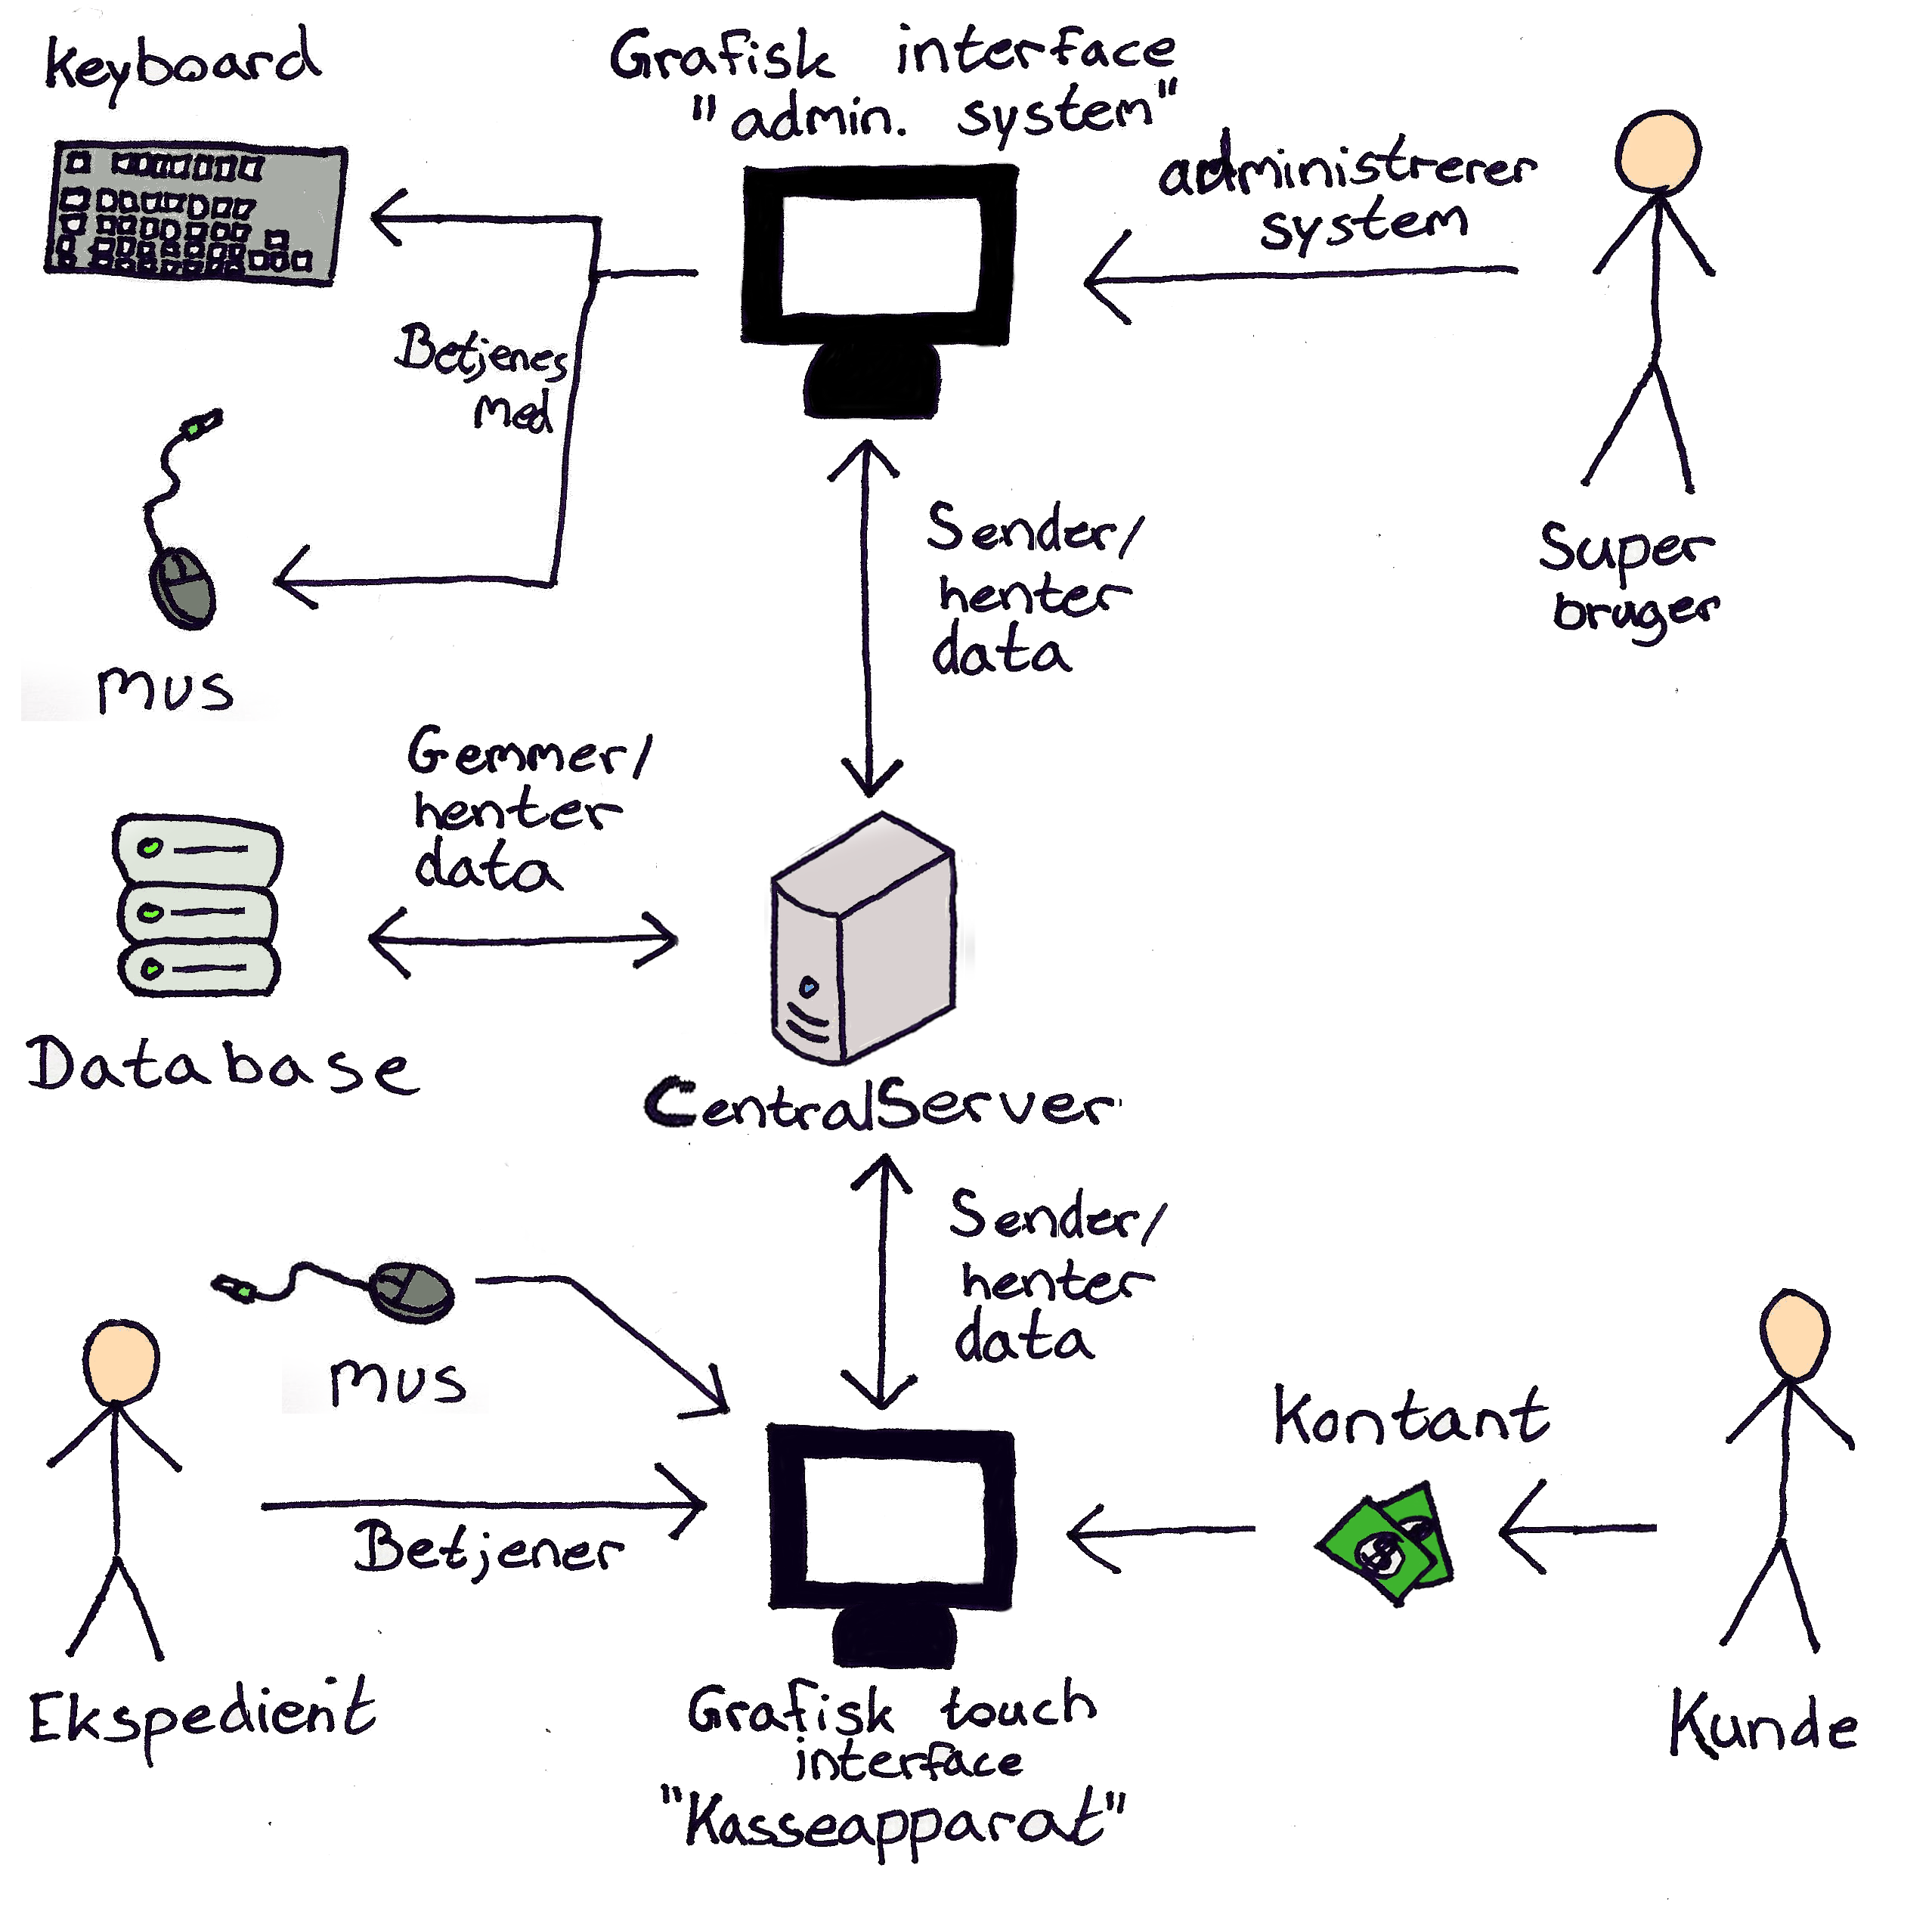
\includegraphics[width=0.8\textwidth]{Systembeskrivelse/RigtBillede3}
    \caption{Rigt billede over Salgssystemet}
    \label{fig:Rigtbill}
\end{figure}